\lecture{4}{27. March 2026}{Performance of Feedback Control Systems}

\section{Performance of Feedback Control Systems}

To really understand the following part on Performance of Feedback Control Systems, a few concepts must first be defined.
\begin{definition}[Transient Response]
  The part of the response that disappears with time.
\end{definition}

\begin{definition}[Steady-State Response]
  The part of the response that exists for a long time following an input signal initiation.
\end{definition}

\begin{definition}[Design Specifications]
  The measures of performance indicating the quality of the system to the designer.
\end{definition}

\subsection{Standard Test Input Signals}
In control theory, we seldom know the exact real-world input a system will see.
Instead, we opt to test the system using simple ``benchmark'' inputs whose responses are easy to analyze.
This helps us answer a lot general questions about the response of a system.
A few of the most common standard test input signals are:
\begin{itemize}
  \item Step Input
  \item Ramp Input
  \item Parabolic Input
  \item Sinusoidal Input
  \item Impulse Input
\end{itemize}

The three most common time-domain test inputs are the step-input, the ramp-input, and the parabolic inputs.
These are all depicted on \Cref{fig:cominpsig}.

\begin{figure} [ht]
  \centering
  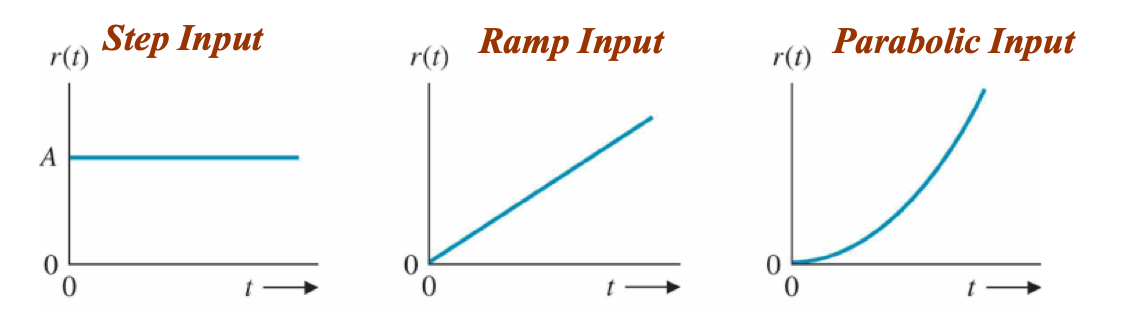
\includegraphics[width=0.5\linewidth]{./figures/cominpsig.png}
  \caption{Common input signals.}
  \label{fig:cominpsig}
\end{figure}

\subsubsection{Step Input} \label{sec:step}
A step input jumps suddenly from 0 to a constant value $A$
\begin{equation*}
  r(t) = A, t >0
\end{equation*}
and its Laplace transform is
\begin{equation*}
  R(s) = \frac{A}{s}
.\end{equation*}
This corresponds to a sudden physical command. Such as setting a motor to a high signal.

\subsubsection{Ramp Input} \label{sec:ramp}
A ramp input grows linearly with time
\begin{equation*}
  r(t) = At, t>0
\end{equation*}
and its Laplace transform is
\begin{equation*}
  R(s) = \frac{A}{s^2}
.\end{equation*}
This corresponds to a steadily changing command, such as asking a vehicle to move forward at constant speed in position coordinates.

\subsubsection{Parabolic Input} \label{sec:par}
A parabolic input grows proportionally to $t^2$
\begin{equation*}
  r(t) = At^2, t>0
\end{equation*}
and its Laplace transform is
\begin{equation*}
  R(s) = \frac{2A}{s^3}
.\end{equation*}
This corresponds to a constantly accelerating command, such as a position reference under constant acceleration.

Worth noting is that the \nameref{sec:ramp} is simply the integral of the \nameref{sec:step}; and the \nameref{sec:par} is the integral of the \nameref{sec:ramp}.

\subsubsection{Unit Impulse Response}
The unit impulse response is defined with regard to the impulse $\delta(t)$.
The ideal impulse is infinitely narrow and infinitely tall, but has area 1 (like an infinitely thin standard normal distribution).
We define this approximately as:
\begin{equation*}
  \delta(t) = \begin{cases}
    \frac{1}{\epsilon}, & - \frac{\epsilon}{2} \leq t \leq \frac{\epsilon}{2}\\
  0, & \text{otherwise}
  \end{cases}
\end{equation*}
as $\epsilon \to 0$.

If the transfer function is $G(s)$, then the system's impulse response is:
\begin{equation*}
  g(t) = \mathcal{L}^{-1} \left\{ G(s) \right\}
.\end{equation*}
This is an extremely important result, as it states that for an LTI system, the impulse response completely characterizes the system.

A convolution is defined as:
\begin{equation*}
  y(t) = \int_{-\infty}^{t} g(t-\tau) r(\tau) \, \mathrm{d}\tau
.\end{equation*}
I.e. the output is the convolution of the input $r(t)$ with the impulse response $g(t)$.
In other words, any input can be built from many tiny impulses, and the output is the sum of the system's response to all those tiny impulses.
In Laplace form this is
\begin{equation*}
  Y(s) = G(s) R(s)
\end{equation*}
which is the transform-domain version of convolution.

\subsubsection{Sinusoidal Input}
The sinusoidal input is defined by
\begin{equation*}
  r(t) = \begin{cases}
    A \sin \omega t, & t \geq 0\\
  0, & t <0
  \end{cases}
\end{equation*}
with Laplace transform:
\begin{equation*}
  R(s) = \frac{A\omega}{s^2  + \omega^2}
.\end{equation*}

\subsubsection{Standard Test Signal Input}
In general, step, ramp, and parabolic inputs can be written as
\begin{equation*}
  r(t) = t^{n}
\end{equation*}
with Laplace transform
\begin{equation*}
  R(s) = \frac{n!}{s^{n+1}}
\end{equation*}


\subsection{Performance of Second-Order Systems}
We consider the general second-order system on \Cref{fig:2ordsys}.
Here, we have the open-loop transfer function
\begin{equation*}
  G(s) = \frac{\omega_n^2}{s(s+ 2\zeta \omega_n}
\end{equation*}
with unity negative feedback.
This results in the closed-loop transfer function becoming
\begin{equation*}
  \frac{Y(s)}{R(s)} = \frac{G(s)}{1+ G(s)} = \frac{\omega_n^2}{s^2 + 2 \zeta \omega_n s + \omega_n^2}
.\end{equation*}

\begin{figure} [ht]
  \centering
  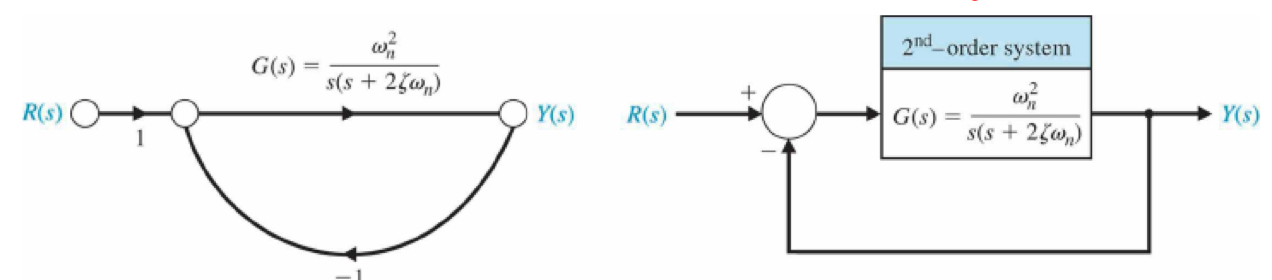
\includegraphics[width=0.8\linewidth]{./figures/2ordsys.png}
  \caption{Second order system.}
  \label{fig:2ordsys}
\end{figure}

Now, we provide the system with a unit step input 
\begin{equation*}
  R(s) = \frac{1}{s}
\end{equation*}
so
\begin{equation*}
  Y(s) = \frac{\omega_n^2}{s \left( s^2 + 2\zeta \omega_n s + \omega_n^2 \right)}
\end{equation*}
and in time domain, for the underdamped case $0 < \zeta < 1$,
\begin{equation*}
  y(t) = 1 - \frac{1}{\beta} e^{- \zeta \omega_n t} \sin \left( \omega_n \beta t + \theta \right)
\end{equation*}
where
\begin{equation*}
  \beta = \sqrt{1 - \zeta^2}, \qquad \theta = \cos^{-1} (\zeta)
.\end{equation*}
This corresponds to a final value of 1 plus an oscillation whose amplitude decays with the exponential term.
The factor
\begin{equation*}
  e^{-\zeta \omega_n t}
\end{equation*}
tells how fast the oscillation dies out, so larger $\zeta$ results in faster decay and less overshoot, whilst smaller $\zeta$ results in slower decay and more ringing.

For the above case, the poles are
\begin{equation*}
  s_{1,2} = - \zeta \omega_n \pm j \omega_n \sqrt{1 - \zeta^2}
.\end{equation*}
Here, $- \zeta \omega_n$ determines how fast the oscillations die out; a more negative real part results in faster decay, and a real part closer to 0 results in slower decay.
The imaginary part
\begin{equation*}
  \omega_n \sqrt{1 - \zeta^2}
\end{equation*}
determines the oscillation frequency, i.e. it is the damped natural frequency
\begin{equation*}
  \omega_d = \omega_n \sqrt{1 - \zeta^2}
.\end{equation*}

The pole plots on \Cref{fig:poleplot}, show how the roots move as $\zeta$ changes.

\begin{figure} [ht]
  \centering
  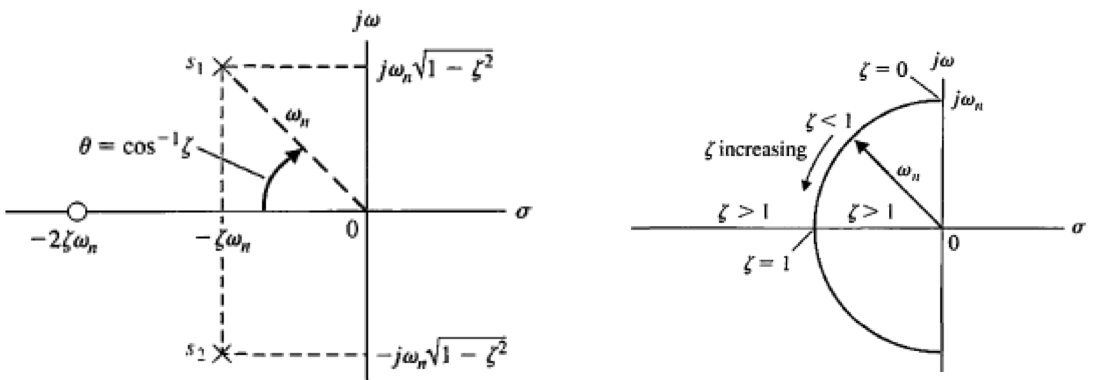
\includegraphics[width=0.8\linewidth]{./figures/poleplot.png}
  \caption{Pole plots}
  \label{fig:poleplot}
\end{figure}

When $0 < \zeta < 1$, the system is underdamped, meaning the poles are complex conjugates
\begin{equation*}
  - \zeta \omega_n \pm j \omega d
.\end{equation*}

When $\zeta = 1$ the system is critically damped.
Here, the two poles meet on the real axis.

When $\zeta > 1$, the system is overdamped.
Here, the poles are real and distinct, and the responds has no oscillation.

For $\zeta = 0$, the system is undamped.
This gives poles on the imaginary axis $\pm j \omega_n$, which correspond to sustained oscillation with no decay.

Also on \Cref{fig:poleplot}, a geometric relationship in the $s$-plane is shown.
For poles of a standard second-order system the distance from the origin is $\omega_n$ and the angle is related to $\zeta$ by
\begin{equation*}
  \cos \theta = \zeta
\end{equation*}
so for fixed $\omega_n$, changing $\zeta$ moves the poles along a circle of radius $\omega_n$.

\begin{figure} [ht]
  \centering
  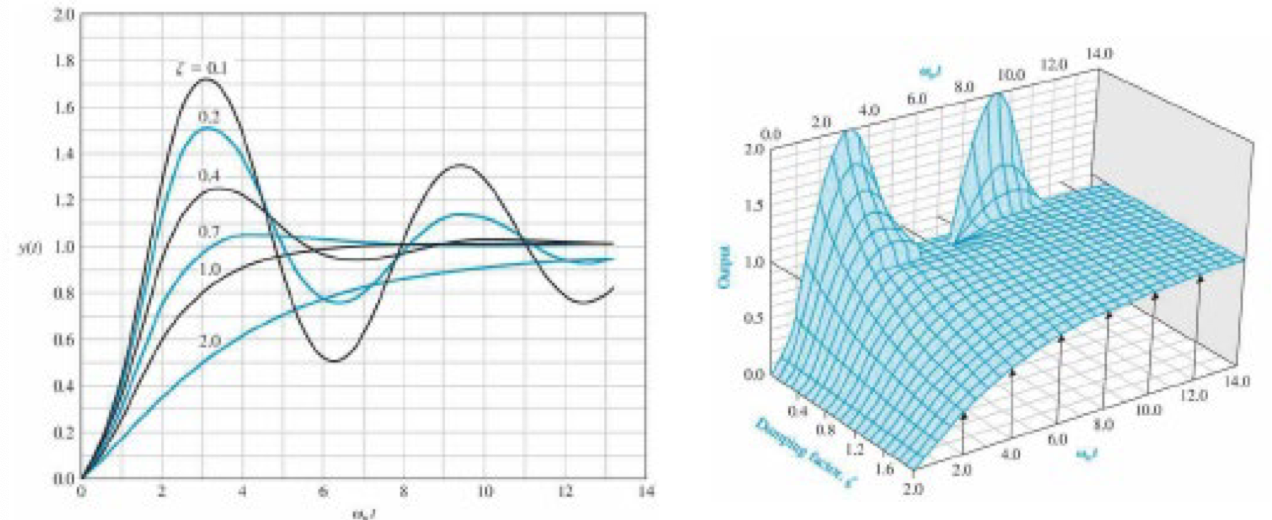
\includegraphics[width=0.8\linewidth]{./figures/timeresps.png}
  \caption{Time responses for different damping ratios}
  \label{fig:timeresps}
\end{figure}

On \Cref{fig:timeresps} the step time response is shown for different damping ratios.
For the small damping ratios, we observe fast initial rise, large overshoot, and strong oscillation.
For the medium damping ratio, we have some overshoot, and less oscillation.
For critical damping, we have no oscillation, and no overshoot.
For the overdamped case, we have no overshoot, and no overshoot, but with a sluggish response.

In general, we can observe that as the damping ratio decreases, the closed-loop roots approach the imaginary axis, and the response becomes increasingly oscillatory.


\subsection{Performance Specification Definition}
On \Cref{fig:perspecdef} a typical step response $y(t)$ approaching its final value $y(\infty)$ is depicted.

\begin{figure} [ht]
  \centering
  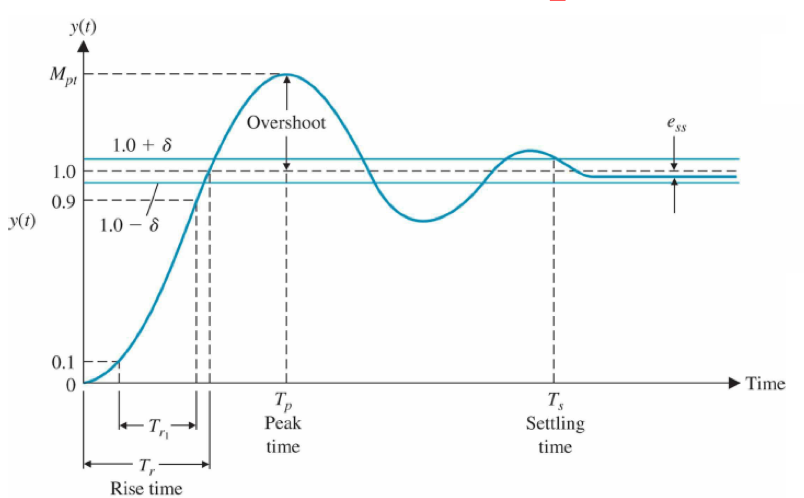
\includegraphics[width=0.5\linewidth]{./figures/perspecdef.png}
  \caption{Typical step response $y(t)$ going toward a final value $y(\infty)$.}
  \label{fig:perspecdef}
\end{figure}

\subsubsection{Rise Time}
We define the rise time on \Cref{fig:perspecdef} as the time it takes the output to ``rise'' to its target value.
For an underdamped system ($\zeta < 1$), the rise time $T_r$ is the first time the response reaches the final value $y(\infty)$.
For an overdamped system ($\zeta > 1$), the response never overshoots, so rise time is often defined as the 10\% to 90\% time:
\begin{equation*}
  T_{r1} = T_2 - T_1
\end{equation*}
with
\begin{equation*}
  y(T_1) = \num{0,1}  y(\infty) , \qquad y(T_2) = \num{0,9} y(\infty)
.\end{equation*}

\subsubsection{Peak Time}
The peak time on \Cref{fig:perspecdef}, is defined as the time, when the response reaches its first maximum.
At the peak, the slope is zero
\begin{equation*}
  \frac{\mathrm{d}y(t)}{\mathrm{d}t} \Bigg|_{t = T_p} = 0
.\end{equation*}
This metric only makes sense for an underdamped response, because overdamped responses do not have a peak above the final value.


\subsubsection{Percent Overshoot}
On \Cref{fig:perspecdef}, the percent overshoot is defined as
\begin{equation*}
  \sigma_p \% = \frac{y(T_p) - y(\infty)}{y(\infty)} \cdot 100 \%
.\end{equation*}
I.e. how much higher than the final value did the first peak go, as a percentage.

For the standard second-order system
\begin{equation*}
  \% \mathrm{OS} = 100 e^{-\zeta \pi\frac{1}{\sqrt{1  - \zeta^2}}}, \qquad 0 < \zeta< 1)
\end{equation*}
I.e. small $\zeta$ leads to lots of oscillation and a large overshoot and vice versa.

\subsubsection{Settling Time}
For an underdamped second-order system, the oscillations decay with an exponential envelope like
\begin{equation*}
  e^{-\zeta \omega_n t}
.\end{equation*}
A few different conventions exist for the settling time, the two most common of which being the 2\% criterion and the 5\% criterion.
If you want your response to be within 2\%, you use
\begin{equation*}
  e^{-\zeta \omega_n T_s} < \num{0,02} 
\end{equation*}
which gives the approximation
\begin{equation*}
  T_s \approx \frac{4}{\zeta \omega_n} = 3\tau
\end{equation*}
for the 2\% criterion, with $\tau = 1 / (\zeta \omega_n)$ being the exponential decay time constant.

Likewise, for the 5\% criterion, a common approximation is
\begin{equation*}
  T_s \approx \frac{3}{\zeta \omega_n} = 3 \tau
.\end{equation*}

\subsubsection{Delay Time}
The delay time, $T_d$ on \Cref{fig:perspecdef}, is defined by
\begin{equation*}
  y(T_d) = \num{0,5} y(\infty)
\end{equation*}
so $T_d$ is the time it takes the output to reach 50\% of its final value. 

\subsubsection{Performance Compromise}
Two important formulas from the above is the formula for the peak time and for the percentage overshoot:
\begin{align*}
  T_P &= \frac{\pi}{\omega_n \sqrt{1 - \zeta^2}} & \%\mathrm{OS} &= 100 e^{-\zeta \pi \frac{1}{\sqrt{1 - \zeta^2}}}
.\end{align*}
These are depicted on \Cref{fig:perfcomp}.
Here we see that, as the damping ratio $\zeta$ increases the percent overshoot decreases and the normalized peak time $\omega_n T_p$ increases, so more damping leads to less overshoot but also a slower response.

\begin{figure} [ht]
  \centering
  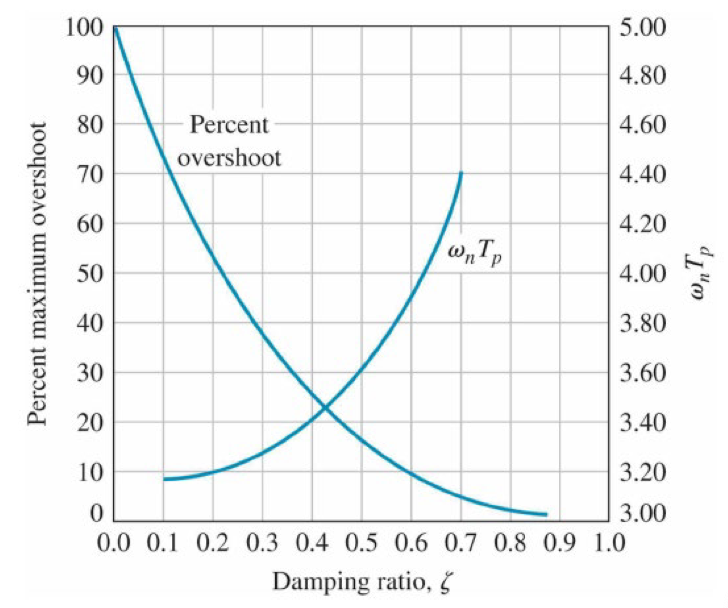
\includegraphics[width=0.5\linewidth]{./figures/perfcomp.png}
  \caption{Performance compromise of control systems.}
  \label{fig:perfcomp}
\end{figure}

This is why a response cannot be made both extremely fast and extremely smooth with no overshoot without changing other elements of the design.

\subsubsection{Swiftness of the System}
On \Cref{fig:swisys1} the normalized rise time $\omega_n T_{r1}$ is plotted versus the damping ratio $\zeta$.
Also present, is a linear approximation of $T_{r1}$ stating:
\begin{equation*}
  T_{r1} \approx \frac{\num{2,16} \zeta + \num{0,60} }{\omega_n}
\end{equation*}
I.e. increasing $\zeta$ increases rise time and increasing $\omega_n$ decreases rise time.

\begin{figure} [ht]
  \centering
  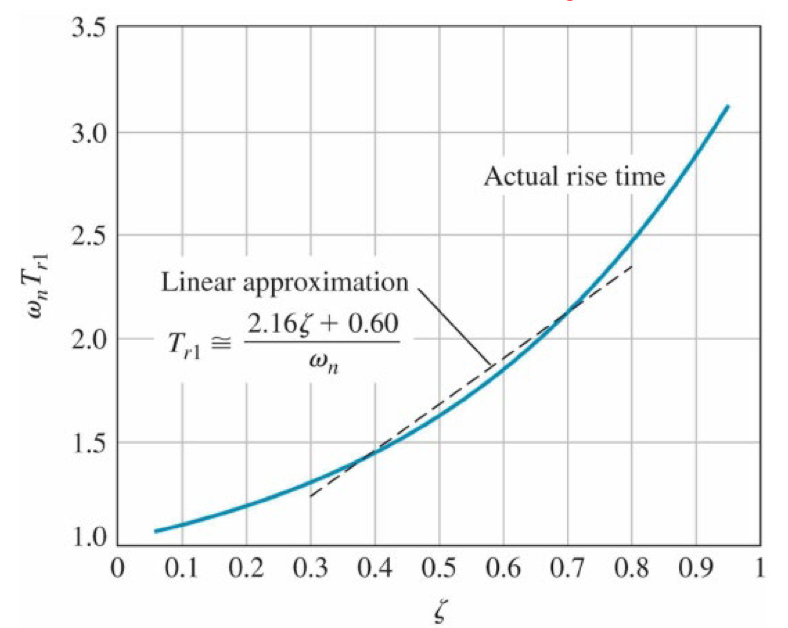
\includegraphics[width=0.5\linewidth]{./figures/swisys1.png}
  \caption{Normalized rise time $\omega_n T_{r1}$ versus $\zeta$ with linear approximation.}
  \label{fig:swisys1}
\end{figure}

\subsection{Effect of a Third Pole}
We consider a third-order system with a closed-loop transfer function:
\begin{equation*}
  T(s) = \frac{1}{\left( s^2 + 2 \zeta s + 1 \right) \left( \gamma s + 1 \right)}
.\end{equation*}
This is basically a second-order part with a complex pole pair and an extra third pole at
\begin{equation*}
  s = - \frac{1}{\gamma}
.\end{equation*}
If that third pole is far enough left in the $s$-plane, it will die out fast and not affect the response much, meaning the system behaves approximately like the second order part.
In the above example, the dominant second-order poles have real part of approximately $- \zeta \omega_n$, and to be able to disregard the influence of the third pole, the dominant pole rule states that
\begin{equation*}
  \left| \frac{1}{\gamma} \right| \geq \left| 10 \zeta \omega_n \right|
\end{equation*}
i.e. the third pole, should be at least 10 times farther left than the real part of the dominant pole pair.
The size of $1 / \gamma$ and therefore the location of the third root changes the settling time and overshoot quite a bit as shown on \Cref{fig:thirdpole}.

\begin{figure} [ht]
  \centering
  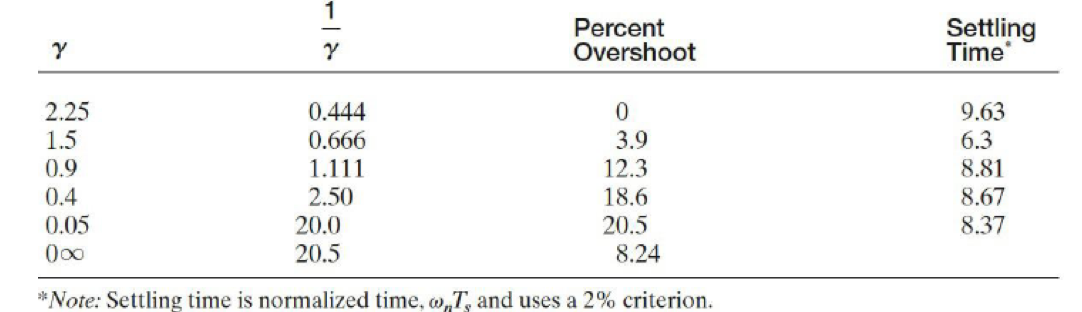
\includegraphics[width=0.8\linewidth]{./figures/thirdpole.png}
  \caption{Effect of a third pole depending on its location.}
  \label{fig:thirdpole}
\end{figure}


\subsection{Effect of a Zero}
We now consider a system with an added zero, with transfer function
\begin{equation*}
  T(s) = \frac{\left( \omega_n^2 / a \right) (s+a)}{s^2 + 2 \zeta \omega_n s + 1}
.\end{equation*}
Here, the extra zero is at $s = -a$.

A zero near the dominant poles can strongly change the transient response.
In other words, if finite zeros are located relatively near the dominant complex poles, they materially affect the transient response.

A zero near the poles typically makes the step response rise faster, overshoot more, and become more ``peaky', as shown on \Cref{fig:zerplot}.

\begin{figure} [ht]
  \centering
  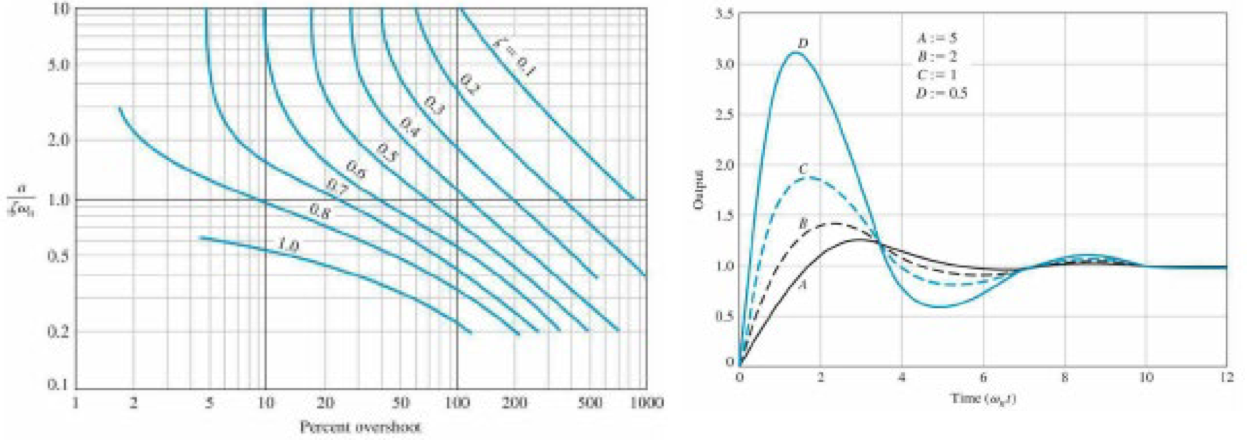
\includegraphics[width=0.8\linewidth]{./figures/zerplot.png}
  \caption{Effect of adding a zero.}
  \label{fig:zerplot}
\end{figure}

Intuitively, a pole stores/slows energy, and a zero tends to add a kind of anticipatory or differentiating effect to this. 

\subsection{Specification Selections}
We consider the system on \Cref{fig:parselex} with forward path
\begin{equation*}
  G(s) = \frac{K}{s(s+p)}
\end{equation*}
and unity feedback, yielding the closed-loop transfer function
\begin{equation*}
  T(s) = \frac{G(s)}{1 + G(s)} = \frac{K}{s^2 + ps + K}
\end{equation*}
which is on the same form as a standard second-order system
\begin{equation*}
  T(s) = \frac{\omega_n^2}{s^2 + 2\zeta \omega_ns + \omega_n^2}
.\end{equation*}

\begin{figure} [ht]
  \centering
  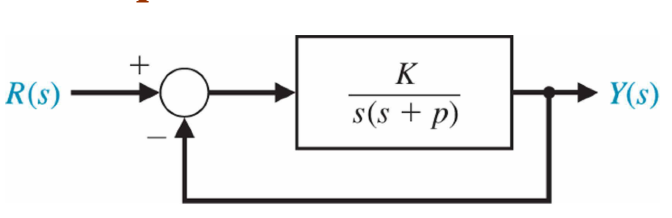
\includegraphics[width=0.8\linewidth]{./figures/parselex.png}
  \caption{Example system.}
  \label{fig:parselex}
\end{figure}

Given this system, we want the step response to have less than 5\% overshoot and a 2\% settling time lower than \qty{4}{\s}.

For a standard second-order system, percent overshoot depends on $\zeta$ by
\begin{equation*}
  \% \mathrm{OS} = 100 e^{- \pi \zeta \frac{1}{\sqrt{1 - \zeta^2}}}
.\end{equation*}
From \Cref{fig:percos}, an overshoot of about \num{4,3} \% corresponds to $\zeta = \num{0,707} $.

\begin{figure} [ht]
  \centering
  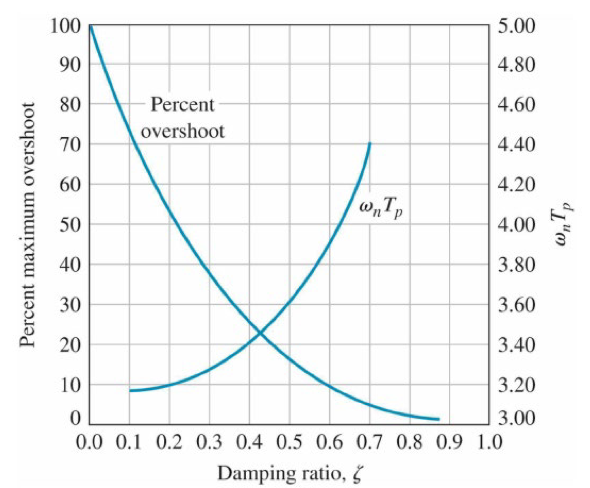
\includegraphics[width=0.5\linewidth]{./figures/percos.png}
  \caption{Percentage overshoot versus damping ratio.}
  \label{fig:percos}
\end{figure}

For the 2\% settling time, the standard approximation is
\begin{equation*}
  T_s \approx \frac{4}{\zeta \omega_n}
.\end{equation*}
We require $T_s \leq  \qty{4}{\s}$, so
\begin{equation*}
  \frac{4}{\zeta \omega_n} \leq 4 \implies \zeta \omega_n \geq 1
.\end{equation*}
This gives the two conditions $\zeta \geq \num{0,707}$ and $\zeta \omega_n \geq 1$.
For a standard underdamped second-order system, the poles are
\begin{equation*}
  s = - \zeta \omega_n \pm j \omega_n \sqrt{1 - \zeta^2}
\end{equation*}
i.e. $\zeta$ controls the angle of the poles and $\zeta \omega_n$ controls the real part.

On the pole plot on \Cref{fig:polzet} the \ang{45} lines correspond to $\zeta = \num{0,707}$ and the vertical line is $\zeta \omega_n = 1$, meaning real part $-1$.
The acceptable region is therefore to the left of $\Re(s) = -1$ inside the wedge corresponding to $\zeta \geq \num{0,707} $

\begin{figure} [ht]
  \centering
  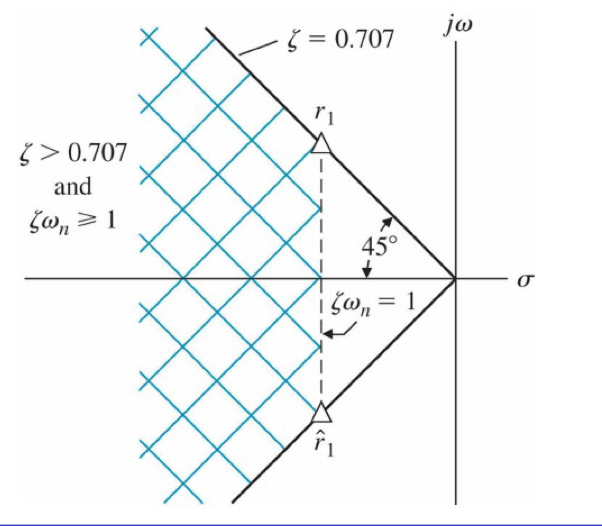
\includegraphics[width=0.5\linewidth]{./figures/polzet.png}
  \caption{Pole plot}
  \label{fig:polzet}
\end{figure}

We choose the boundary case $\zeta = \num{0,707}, \zeta\omega_n = 1$, so
\begin{equation*}
  \omega_n = \frac{1}{\zeta} = \frac{1}{\num{0,707}} = \sqrt{2}
.\end{equation*}
From earlier
\begin{equation*}
  T(s) = \frac{K}{s^2 + ps + K}
.\end{equation*}
Comparing this with
\begin{equation*}
  \frac{\omega_n^2}{s^2 + 2\zeta \omega_n s + \omega_n^2}
.\end{equation*}
Matching coefficients gives
\begin{equation*}
  K = \omega_n^2, \qquad p = 2 \zeta \omega_n
.\end{equation*}
Substituting, we get:
\begin{equation*}
  K = \left( \sqrt{2} \right)^2 = 2
\end{equation*}
and since $\zeta \omega_n = 1$, $p = 2 \zeta \omega_n = 2$, so
\begin{equation*}
  K = 2, \qquad p = 2
.\end{equation*}

\subsubsection{Estimating the Damping Ratio}
The dampind ratio, $\zeta$, can be estimated, just by looking at a step response.
In general the number of visible oscillations is:
\begin{equation*}
  \text{Cycles visible} = \frac{4\beta}{2\pi \zeta} \approx \frac{\num{0,55} }{\zeta}
.\end{equation*}
So approximately
\begin{equation*}
  \zeta \approx \frac{\num{0,55} }{\text{cycles visible}}
.\end{equation*}


\subsection{s-Plane Root Location and Transient Response}
A transfer-function response can be decomposed into terms like
\begin{equation*}
  \frac{A_i}{s + \sigma_i} \quad \text{and}\quad \frac{B_k s + C_k}{s^2 + 2 \alpha_k s + \left( \alpha_k^2 + \omega_k^2 \right)}
.\end{equation*}
In time domain these become real exponential terms like $e^{-\sigma t}$ and oscillatory ones like $e^{-\alpha t} \sin \left( \omega t + \theta \right)$.
The step-response of different root locations in the $s$-plane is shown on \Cref{fig:impres}.

\begin{figure} [ht]
  \centering
  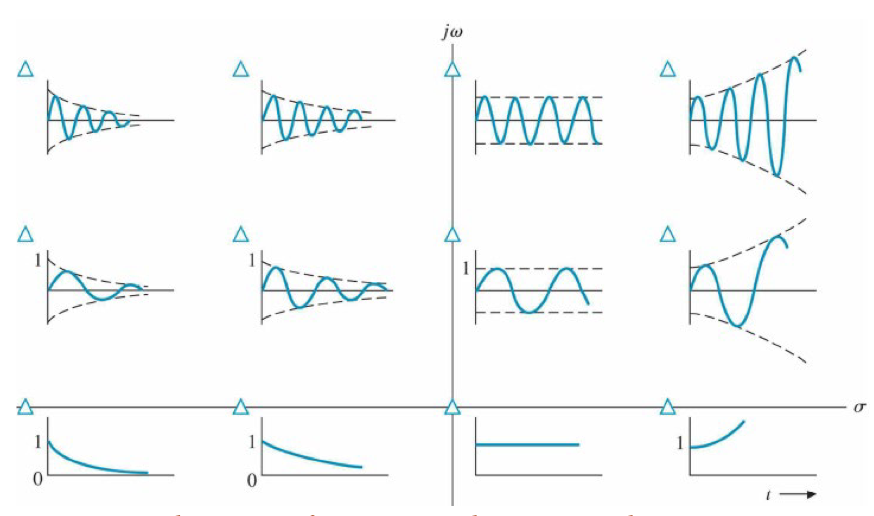
\includegraphics[width=0.6\linewidth]{./figures/impres.png}
  \caption{Impulse response for various root locations in $s$-plane}
  \label{fig:impres}
\end{figure}

On the $s$-plane, poles are at $s = \sigma + j \omega$, the real part $\sigma$ decides whether the response decays ($\sigma < 0$), stays constant ($\sigma = 0$), or grows $(\sigma >0)$.
The imaginary part gives oscillation frequency.


\subsection{Steady-state Error}
We consider the system on \Cref{fig:steadyerr} with:
\begin{itemize}
  \item Reference input $R(s)$
  \item Error $E_a (s)$
  \item Controller $G_C (s)$
  \item plant $G(s)$
  \item Output $Y(s)$
\end{itemize}
Because of unity feedback,
\begin{equation*}
  E(s) = R(s) - Y(s)
\end{equation*}
and since
\begin{equation*}
  Y(s) = G_C(s) G(s) E(s)
\end{equation*}
we get
\begin{equation*}
  E(s) = \frac{1}{1 + G_C (s) G(s) }R(s)
.\end{equation*}
This is the error-transfer formula.

\begin{figure} [ht]
  \centering
  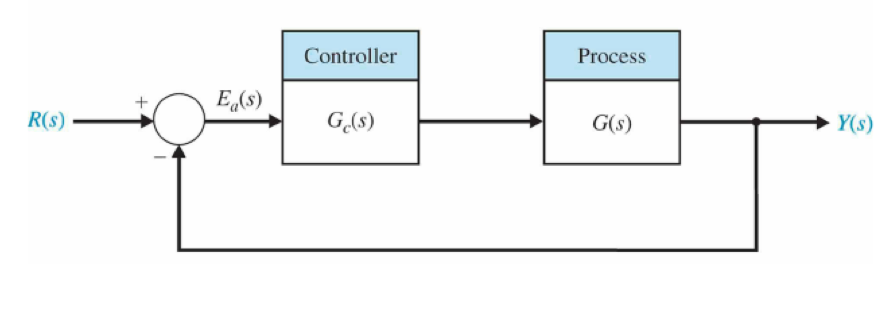
\includegraphics[width=0.8\linewidth]{./figures/steadyerr.png}
  \caption{Example unity-feedback control system.}
  \label{fig:steadyerr}
\end{figure}

The steady-state error is the error after the transient has died out:
\begin{equation*}
  e_{ss} = \lim_{t \to \infty}e(t)
.\end{equation*}
Using the final value theorem:
\begin{equation*}
  e_{ss} = \lim_{s \to 0} s E(s)
.\end{equation*}
So, with the previous expression for $E(s)$
\begin{equation} \label{eq:ss}
  e_{ss} = \lim_{s \to 0}s \cdot \frac{1}{1 + G_c(s) G(s)}R(s)
.\end{equation}
Here, it is worth noting that $s \to 0$ means low-frequency / DC-behavior, so steady-state error depends on the system's behavior near $s = 0$.

\subsubsection{Steady-State Error for Step Input}
For a stem of magnitude $A$,
\begin{equation*}
  r(t) = A \qquad \implies \qquad R(s) = \frac{A}{s}
.\end{equation*}
Plugging this into \Cref{eq:ss} we get:
\begin{equation*}
  e_{ss} = \lim_{s \to 0} s \frac{1}{1 + G_C(s) G(s)} \cdot \frac{A}{s} = \frac{A}{1 + \lim_{s \to 0} G_C(s) G(s)}
.\end{equation*}
So, the step error depends on the DC loop gain.

The loop transfer function is written generally as:
\begin{equation*}
  G_C(s) G(s) = \frac{K \prod_{i = 1}^{M} (s + z_i)}{S^{N} \prod_{k = 1}^{Q} (s + p_k)}
.\end{equation*}
The $S^{N}$ factor in the denominator ensures we have $N$ poles at the origin, i.e. $N$ \textit{pure integrators}.
This $N$ is called the type number.

For a type 0 system ($N = 0$), $G_C(s) G(s)$ stays finite as $s \to 0$.
We define the position error constant as
\begin{equation*}
  K_p = \lim_{s \to 0} G_c(s) G(s)
\end{equation*}
then
\begin{equation*}
  e_{ss} = \frac{A}{1 + K_p}
.\end{equation*}
Meaning a type-0 system usually has a nonzero constant error to a step.
Increasing low-frequency gain increases $K_p$, which reduces error, but it does not make it zero.

If the system has one or more integrators ($N \geq 1$), then $\lim_{s \to 0} G_C(s) G(s) = \infty$, so
\begin{equation*}
  e_{ss} = 0
\end{equation*}
for a step input.
So, type-0 will have a finite step error and type-1 or higher will have zero step error.

\subsubsection{Steady-State Error for Ramp Input}
For a ramp with slope $A$,
\begin{equation*}
  r(t) = A(t) \qquad \implies R(s) = \frac{A}{s^2}
\end{equation*}
then \Cref{eq:ss} becomes
\begin{equation*}
  e_{ss} = \lim_{s \to 0}s \cdot \frac{1}{1 + G_C(s) G(s)} \cdot \frac{A}{s^2}
,\end{equation*}
which simplifies to a behavior controlled by $\lim_{s \to 0} s G_C(s) G(s)$.
We now define the velocity error constant
\begin{equation*}
  K_v = \lim_{s \to 0}s G_C(s) G(s)
\end{equation*}
then for a type-1 system,
\begin{equation*}
  e_{ss} = \frac{A}{K_v}
.\end{equation*}

A type-0 system has no integrator, then as $s G_C(s) G(s) \to 0$, $e_{ss} = \infty$, meaning a type-0 system cannot follow a ramp forever, the error keeps growing infinitely.

For a type-1 system $K_v$ is finite, so
\begin{equation*}
  e_{ss} = \frac{A}{K_v}
,\end{equation*}
meaning the output follows the ramp with the same slope, but with a constant offset.

A type-2 or higher system will mean $K_v \to \infty$, so
\begin{equation*}
  e_{ss} = 0
\end{equation*}
meaning type-2+ can track a ramp perfectly in steady-state.

\subsubsection{Steady-State Error for Accelerating/Parabolic Input}
Here, the input is
\begin{equation*}
  r(t) = \frac{At^2}{2} \qquad \implies \qquad R(s) = \frac{A}{s^3}
\end{equation*}
meaning the relevant term is
\begin{equation*}
  \lim_{s \to 0} s^2 G_C(s) G(s)
.\end{equation*}
We now define the acceleration error constant $K_a = \lim_{s \to 0} s^2 G_C(s) G(s)$, and for a type-2 system we get, by insertion into \Cref{eq:ss}:
\begin{equation*}
  e_{ss} = \frac{A}{K_a}
.\end{equation*}

For a type-0 or type-1 system we do not have enough integrators to track a parabolic input so $e_{ss} = \infty$.

A type-2 system gives two integrators, so
\begin{equation*}
  e_{ss} = \frac{A}{K_a}
\end{equation*}
corresponding a constant finite error.

Type-3 or higher systems, gives
\begin{equation*}
  e_{ss} = 0
\end{equation*}
corresponding to a perfect steady-state tracking of a parabolic input.

\subsection{Performance Indices}
A performance index is a single number used to measure how good or bad a system response is.
Usually in control, we care about how large the error is, how long the error lasts, how much overshoot there is, how quickly the system settles, etc.
Instead of judging all of these from a graph, we define a mathematical quantity based on the error $e(t)$, and then try to minimize it, so a small performance index corresponds to a better response and a large performance index corresponds to a worse response.

An optimum control system is one where the system parameters are chosen so that the chosen performance index becomes as small as possible.
E.g. one might tune controller gains, $K_p$, $K_i$, $K_d$, so that one of these errors is minimized.

All of the indices are based on the tracking error
\begin{equation*}
  e(t) = r(t) - y(t)
\end{equation*}

Some common performance indices are presented in the following parts.

\subsubsection{Integral of the Square of the Error (ISE)}
The integral of the square of the error, is defined as
\begin{equation*}
  \mathrm{ISE} = \int_{0}^{T} e^2(t) \, \mathrm{d}t 
\end{equation*}
meaning you square the error and add it up over time.
This tends to favor responses that reduce large errors quickly, but as small errors are not weighted as much oscillation is not impeded much.

\subsubsection{Integral of the Absolute Error (IAE)}
The integral of the absolute error, is defined as
\begin{equation*}
  \mathrm{IAE} = \int_{0}^{T} \left| e(t) \right|\, \mathrm{d}t 
\end{equation*}
meaning you take the absolute value of the error and add it over time.
This does not exaggerate large errors as much as ISE and generally treats errors more ``linearly''.

\subsubsection{Integral of Time Multiplied by Absolute Error (ITAE)}
The integral of the time multiplied by absolute error, is defined as
\begin{equation*}
  \mathrm{ITAE} = \int_{0}^{T} t \left| e(t) \right| \, \mathrm{d}t 
\end{equation*}
meaning the absolute error is now multiplied by the time $t$ before being integrated.
I.e. errors at the beginning count less and errors later count more.
This generally helps to reduce settling time and long-lasting oscillation.

\subsubsection{Integral of Time multiplied by the Squared Error (ITSE)}
The integral of time multiplied bu the squared error is defined as
\begin{equation*}
  \mathrm{ITSE} = \int_{0}^{T} te^{2}(t) \, \mathrm{d}t
.\end{equation*}
This combines the ideas of squaring the error to emphasise large errors, and multiplying by the time to emphasise late errors.

\subsubsection{The factor T}
The factor $T$ in all the above integrals is usually chosen as the settling time $T_s$.
This means the integral is often evaluated only over a practical time window.
In theory, people sometimes also use
\begin{equation*}
  \int_{0}^{\infty} \ldots \, \mathrm{d}t 
\end{equation*}
if the response dies out and the integral remains finite.

\subsubsection{Simplification of Linear Systems}
We have two main methods if we want to approximate a high-order transfer function as a lower-order one that keeps the most important behavior.

The first method is deleting an insignificant pole.
E.g.
\begin{equation*}
  G(s) = \frac{K}{s(s+2)(s+30)}
\end{equation*}
with poles at $s = 0, -2, -30$.
Here the pole at $-30$ corresponds to a very fast mode that dies out much faster than the other two, so for the slower response, we approximate
\begin{equation*}
  s + 30 \approx 30
\end{equation*}
which gives
\begin{equation*}
  G(s) \approx \frac{K}{30s (s+2)} = \frac{K / 30}{s (s+2)}
.\end{equation*}
This is called a \textit{dominant-pole approximation}.

The second method is matching the frequency response.
Instead of just deleting a pole, you can instead build a lower-order model whose frequency response is close to the original one.
Say for a high-order system
\begin{equation*}
  G_H (s) = K \frac{a_m s^{m} + a_{m-1} s^{m-1} + \ldots + a_1 s + 1}{b_n s^{n} + b_{n-1}s^{n-1}+\ldots +b_1s+1}
\end{equation*}
we can create a lower-order approximation
\begin{equation*}
G_L (s) = K \frac{c_p s^{p} + \ldots + c_1 s + 1}{d_q s^{q} + \ldots  + d_1s + 1}
\end{equation*}
by choosing the $c_i$ and $d_i$ so that $G_L(s)$ behaves as much like $G_H(s)$ as possible in frequency.
In general, to match frequency response, the ratio
\begin{equation*}
  \frac{G_H(s)}{G_L(s)} = \frac{M(s)}{\Delta (s)} \to 1
\end{equation*}
I.e. if $G_L(s)$ is a good approximation, then the ratio $G_H(s) / G_L(s)$ should be close to 1.
So the goal is to make the numerator and denominator of that ratio behave similarly.
We can match using,
\begin{equation*}
  M_{2q} = \Delta_{2q}
\end{equation*}
for $q = 0,1,2,\ldots $
I.e. you compare certain coefficients derived from $M(s)$ and $\Delta(s)$ and force them to be equal.

\begin{exa}[Frequency Response Matching]
  We seek to approximate the system
  \begin{equation*}
    G_H(s) = \frac{6}{s^3 + 6s^2 + 11s + 6}
  \end{equation*}
  by a second-order model
  \begin{equation*}
    G_L(s) = \frac{1}{1 + d_1 s + d_2 s^2}
  .\end{equation*}
  \tcblower
  We start by dividing the denominator by 6
  \begin{equation*}
    G_H(s) = \frac{1}{1 + \frac{11}{6} s + s^2 + \frac{1}{6}s^3}
  .\end{equation*}
  Now, we define
  \begin{equation*}
    \Delta (s) = 1 + \frac{11}{6}s + s^2 + \frac{1}{6}s^3
  \end{equation*}
  and for the approximate model
  \begin{equation*}
    M(s) = 1 + d_1s + d_2s^2
  \end{equation*}
  because
  \begin{equation*}
    \frac{G_H(s)}{G_L(s)} = \frac{1 / \Delta (s)}{1 / M(s)} = \frac{M(s)}{\Delta (s)}
  .\end{equation*}
  
  Now we compute the derivatives at $s = 0$.
  For $\Delta (s)$:
  \begin{equation*}
    \Delta^{(0)}(0) = 1, \quad \Delta^{(1)}(0) = \frac{11}{6}, \quad \Delta^{(2)}(0) = 2, \quad \Delta^{(3)}(0) = 1
  \end{equation*}
  and for $M(s)$:
  \begin{equation*}
    M^{(0)} (0) = 1, \quad M^{(1)}(0) = d_1, \quad M^{(2) }(0) = 2d_2, \quad M^{(3) }(0) = 0
  .\end{equation*}
  
  Now, we match the coefficients, by first computing
  \begin{equation*}
    M_2 = d_1^2 - 2d_2
  \end{equation*}
  and
  \begin{equation*}
      \Delta_2 = \frac{49}{36}
  .\end{equation*}
  So matching gives
  \begin{equation*}
    d_1^2 - 2d_2 = \frac{49}{36}
  .\end{equation*}
  The next matching condition gives
  \begin{equation*}
    M_4 = \Delta_4
  \end{equation*}
  which becomes
  \begin{equation*}
    d_2^2 = \frac{7}{18} \implies d_2 \approx \num{0,624}  \implies d_1 \num{1,615} 
  .\end{equation*}
  So
  \begin{equation*}
    G_L(s) \approx \frac{1}{1 + \num{1,615} s + \num{0,624} s^2}
  .\end{equation*}
\end{exa}
